\documentclass[12pt]{beamer}

\usetheme{Oxygen}
\usepackage{graphicx}
\usepackage{thumbpdf}
\usepackage{wasysym}
\usepackage{ucs}
\usepackage[utf8]{inputenc}
\usepackage{pgf,pgfarrows,pgfnodes,pgfautomata,pgfheaps,pgfshade}
\usepackage{verbatim}


\pdfinfo
{
  /Title       (Les GUI avec Qt)
  /Creator     (Emmanuel Guiraud ~ Quentin Philippot)
  /Author      (Emmanuel Guiraud ~ Quentin Philippot)
} 


\title{Les GUI avec Qt}
\author{Emmanuel Guiraud~-~Quentin Philippot}
\date{16 Octobre 2014}

\begin{document}

\frame{\titlepage}

\section*{}
    \begin{frame}{Sommaire}
        \tableofcontents[section=1,hidesubsections]
    \end{frame}
\AtBeginSection[]
{
  \frame<handout:0>
  {
    \frametitle{Sommaire}
    \tableofcontents[currentsection,hideallsubsections]
  }
}

\AtBeginSubsection[]
{
  \frame<handout:0>
  {
    \frametitle{Sommaire}
    \tableofcontents[sectionstyle=show/hide,subsectionstyle=show/shaded/hide, subsubsectionstyle=show/shaded/hide]
  }
}

\newcommand<>{\highlighton}[1]{%
  \alt#2{\structure{#1}}{{#1}}
}

\newcommand{\icon}[1]{\pgfimage[height=1em]{#1}}



%%%%%%%%%%%%%%%%%%%%%%%%%%%%%%%%%%%%%%%%%
%%%%%%%%%% Content starts here %%%%%%%%%%
%%%%%%%%%%%%%%%%%%%%%%%%%%%%%%%%%%%%%%%%%

%////////////////////////   INTRO   ////////////////////////////

\section{Graphical User Interface}
    \subsection{Ce que n'est pas une GUI}
        \begin{frame}{CLI : Console, très chère console ...}
        \begin{block}{Command Line Interface}
            La plus ancienne des interfaces conversationnelles développées sur des ordinateurs. Avant cela, c'était le règne des cartes perforées.\\\textbf{Aujourd'hui :} utilisation du terminal.
        \end{block}
        
        \end{frame}
       \begin{frame}{Command Line Interface}
       
     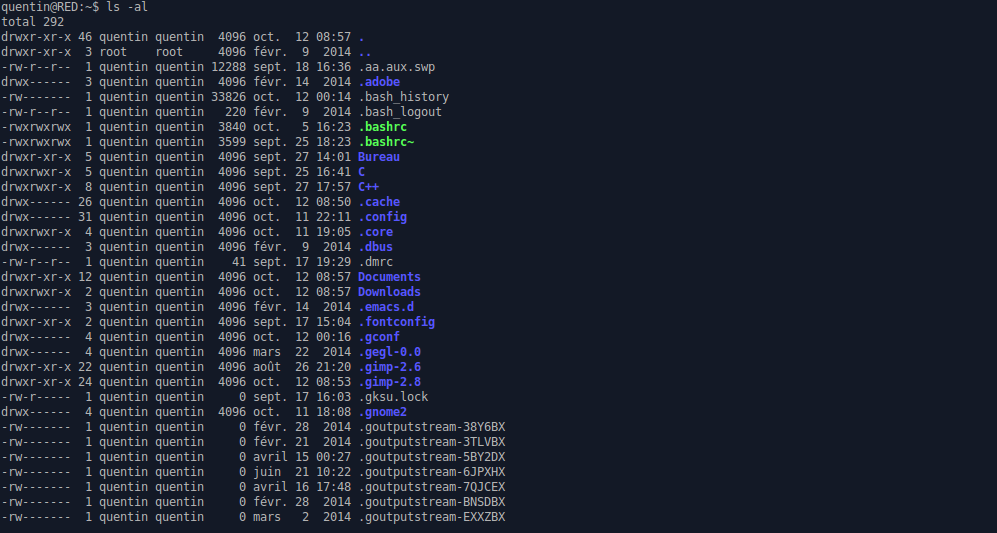
\includegraphics[width=1\textwidth]{pictures/cli.png}
        \end{frame}
    
        \begin{frame}{TUI : Une avancée visuelle}
            \begin{block}{Text User Interface }
            Ce n'est pas encore une GUI, mais elle possède néanmoins des fenêtres, est capable de générer des pop-up et possède un système rudimentaire de menu déroulant. Les interactions se font avec le clavier et la souris.\\\textbf{Aujourd'hui :} Menu BIOS, par exemple.
            \end{block}
       \end{frame}
       
\begin{frame}{Text User Interface}
    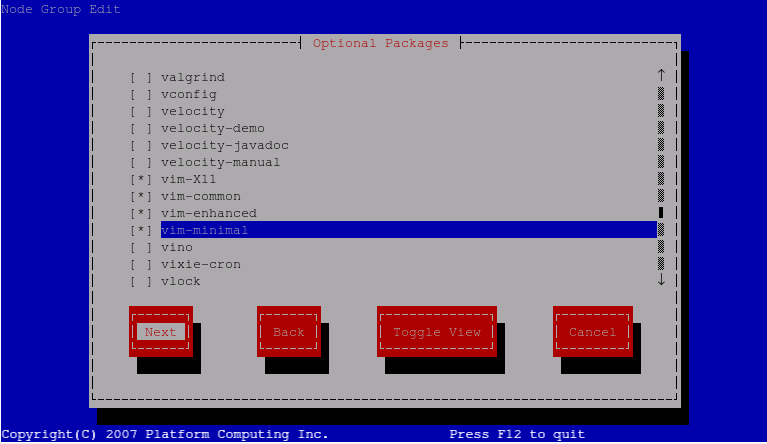
\includegraphics[width=1\textwidth]{pictures/TUI.png}
    \end{frame}
    \subsection{Ce qu'est une GUI}
    
        \begin{frame}{Mais qu'est-ce qu'une GUI ?}
            \begin{block}{Graphical User Interface}
  Les fenêtres telles que nous les connaissons. Les objets sont affichés sous forme de pictogramme. 
                \begin{itemize}
                    \item Interface la plus \textbf{user-friendly}: objectif rendre l'interaction avec le système transparente.
                    \item L'écriture d'une commande complexe est remplacée par un simple clic ou la pression d'une touche.
                \end{itemize}
                \textbf{Aujourd'hui :} La majorité des interfaces sont des GUI !
            \end{block}
        \end{frame}
        
           \begin{frame}{Graphical User Interface}
       
     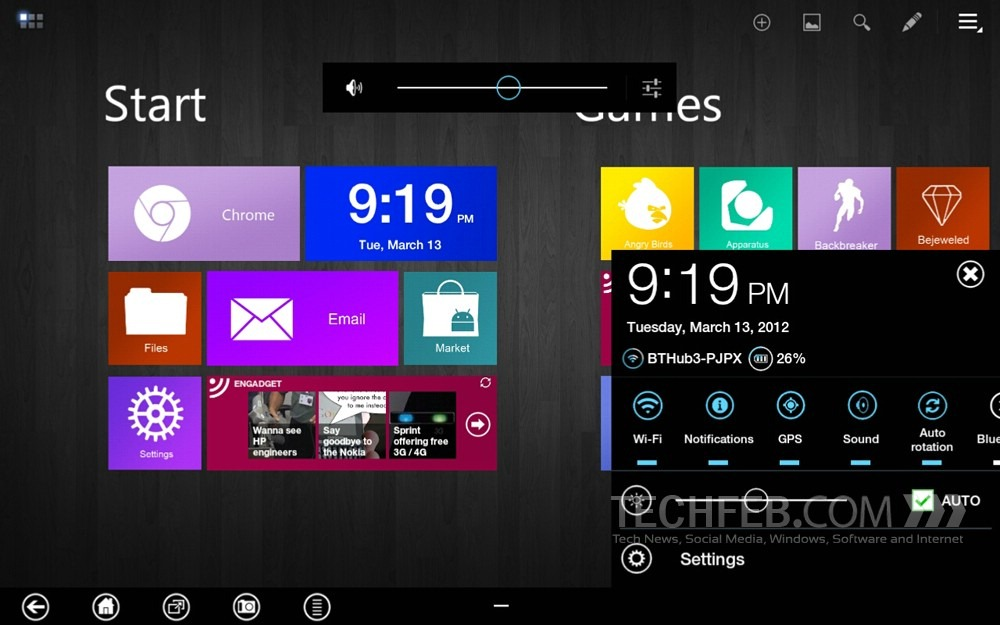
\includegraphics[width=1\textwidth]{pictures/gui.png}
        \end{frame}
    
    %//////////////////  QT  ////////////////////////
        
\section{La bibliothèque graphique Qt}
    \subsection{Qu'est-ce que Qt ?}
        \begin{frame}{Qu'est-ce que Qt ?}
            \begin{itemize}
                \item{C'est un \textbf{Framework} : un ensemble de bibliothèques\\(plus de 13Go !)}
                \item{Projet débuté en 1991 par Trolltech, repris aujourd'hui par Qt-Project.}
                \item{Permet de créer des programmes sous licence LGPL ou propriétaire.}
                \item{Surcouche du C++ (livré avec un IDE et un gestionnaire de surcouche).}
                \item{Multi-plateformes.}
            \end{itemize}
        \end{frame}
        
    
    %//////////////////  WIDGETS   ////////////////////////////
    
    \subsection{Le monde des Widgets} 
            \begin{frame}{Les Widgets}{Qu'est-ce qu'un Widget? (Window Gadget)}
                \begin{itemize}
                    \item{C'est la brique de nos fenêtres Qt.}
                    \item{En pratique, tout type de widget est une spécialisation de \textit{QWidget} :}
                    \begin{itemize}
                        \item{Les layouts (\textit{QLayout})}
                        \item{Les champs d'édition de texte (\textit{QLineEdit})}
                        \item{Les boutons (\textit{QButton})}
                        \item{Et bien d'autres encore...}
                    \end{itemize}
                \end{itemize}
            \end{frame}

    
            \begin{frame}{Les Layouts}{L'agencement des widgets}
                Comment organiser sa fenêtre ?
                \begin{block}{Les Layouts}
                    Il s'agit d'un widget dédié à l'organisation spatiale : c'est un \textbf{conteneur} qui ordonne son contenu suivant ses spécificités, et de manière transparente pour l'utilisateur.\\On retrouve notamment:
                    \begin{itemize}
                      \item{les layouts horizontaux }
                      \item{les layouts verticaux}
                      \item{les layouts de grille}
                       \item{les layouts de formulaire}
                       \item{les layouts piles}
                 \end{itemize}
                \end{block}
            \end{frame} 
            
            \begin{frame}{Les Layouts}{L'emboîtement}
                Comment utiliser les layouts ?
                \begin{block}{Propriété des Layouts}   
                    Un layout peut contenir n'importe quel type de widget.\\Il peut donc contenir d'autres layouts.
                \end{block}
                \begin{block}{Principe de l'emboîtement}
                    Un layout ne peut gérer qu'une mise en forme à la fois, il suffit alors d'imbriquer plusieurs layouts pour parvenir à une mise en forme plus complexe.
                \end{block}
            \end{frame}
            
                            
            \begin{frame}{Les Layouts}{Illustration}
            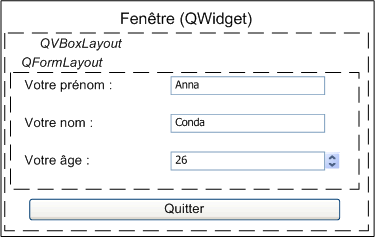
\includegraphics[width=1\textwidth]{pictures/Layout.png}
            \end{frame}
            
            \begin{frame}{Interagir avec sa fenêtre}{Les boutons}
                Comment créer le lien entre l'interface et notre programme ?
                \begin{block}{Les types de boutons}
                    Il existe plusieurs types de boutons fourni par Qt, chacun répondant a un besoin spécifique :
                    \begin{itemize}
                    \item{Les boutons cliquables}
                    \item{Les cases à cocher}
                    \item{Les boutons de barre d'outils}
                    \item{Et d'autres encore...}
                    \end{itemize}
                \end{block}
            \end{frame}
            
            \begin{frame}{Interagir avec sa fenêtre}{Les champs de texte}
                Comment afficher/recevoir des informations ?
                \begin{block}{Les champs d'affichage}
                    Il existe plusieurs champs d'affichages :
                    \begin{itemize}
                    \item{Les champs de texte}
                    \item{Les champs de lecture}
                    \item{Les champs d'images}
                    \end{itemize}
                \end{block}
                \begin{block}{Les champs d'écriture}
                    On n'utilise qu'un seul widget en général : \textit{QLineEdit}.\\ Ses propriétés le rendent très souple : on peut ainsi masquer les caractères entrés, modifier la taille du champ, limiter la longueur du texte à écrire...
                \end{block}
            \end{frame}
            
            \begin{frame}{Interagir avec sa fenêtre}{Pour aller plus loin}
                Lorsque que notre GUI commence à se complexifier, on peut avoir besoin d'avoir besoin de plus d'options/fonctionnalités.
                \begin{block}{Les menus}
                    Contrairement aux widgets vus jusqu'à présent, les menus ne sont pas pré-implémentés : c'est à l'utilisateur de spécifier les noms de menus, les options proposées, leurs actions, et autres propriétés (raccourcis clavier, par exemple.)
                \end{block}
                \begin{block}{La personnalisation}
                    Qt reposant sur la POO, il est ainsi possible de créer ses propres widgets héritant de widgets préexistants.
                \end{block}
            \end{frame}
            
            
            
    %//////////////////  EVENEMENTS  //////////////////////////

    
    \subsection{Programmation Événementielle}
        \subsubsection{Principe général}
            \begin{frame}{Interagir avec la GUI}{Quel moyen ?}
                \begin{itemize}
                    \item{Comment communiquer avec notre interface ?}
                \end{itemize}
                \begin{block}{On utilise des événements}
                        Ce sont des "messages" envoyés par un périphérique (ou le système d'exploitation) à l'application. \\Quelques exemples d'événements :
                        \begin{itemize}
                            \item{L'utilisateur presse une touche du clavier.}
                            \item{Il bouge la souris.}
                            \item{Il réduit la fenêtre.}
                        \end{itemize}
                        \textbf{Remarque :} Qt nomme ses événements \textit{QEvent}.
                    \end{block}
                \end{frame}
        
                \begin{frame}{Interagir avec la GUI}{Des événements, et ensuite ? }
                    \begin{itemize}
                        \item{Comment intercepter/traiter les événements reçus ?}
                    \end{itemize}
                    \begin{block}{On utilise une boucle principale (ou \textbf{mainloop})}
                        \begin{itemize}
                            \item{Tout d'abord, le système place les événements dans une file (transparent pour le programmeur).}
                            \item{Puis on récupère l'événement en tête de file, le traite, et réitère jusqu'à ce qu'un événement de fin mette un terme à la boucle.}
                        \end{itemize}
                    \end{block}
                \end{frame}
                
                \begin{frame}{Exemple (1)}{mainLoop}
                    \textbf{mainLoop() :}
                    \begin{verbatim}
                    %indenter pseudo code
                    Faire evenementCourant := recupererEvenement()\\
                    |~~~si evenementCourant == evenement_1\\
                    |~~~|~~~~alors traitement prévu pour evenement_1\\
                    |~~~si evenementCourant == evenement_2\\
                    |~~~|~~~alors traitement prévu pour evenement_2\\|\\
                    |~~~... On étudie chaque cas de figure ...\\|\\
                    tant que evenementCourant != evenementFin
                    \end{verbatim}
                \end{frame}
        
                \begin{frame}{Exemple (2)}{code programme}
                Le code de notre programme devient :\\ 
                \textbf{Programme :}
                    \begin{verbatim}
                        ~~definirGUI() //Structuration avec widgets\\
                        ~~mainLoop()
                    \end{verbatim}
                    \begin{block}{Constat}
                        La programmation événementielle dans la boucle principale est très lourde (il faut prévoir chaque cas de manière exhaustive, et déterminer un traitement spécifique.)
                    \end{block}
                \end{frame}
                
       \subsubsection{Les signaux et les slots}
            \begin{frame}{Programmation Événementielle}{Les deux mécanismes}
            Qt propose deux mécanismes parallèles pour traiter les événements :
            \begin{itemize}
            \item le traitement des \textit{QEvent}.
            \item Un mécanisme de signaux et de slots.
            \end{itemize}
            \end{frame}
            \begin{frame}{Les signaux et les slots}
                \begin{block}{Les signaux}
                    Les signaux sont simplement des messages qui peuvent être connectés à des actions que nous voulons exécuter.
                \end{block}
                \begin{block}{les slots}
        Les slots sont des fonctions (ou méthodes) qui exécutent un traitement.\\Les slots sont connectés à des signaux qui les appellent.
    \end{block}
    
    \end{frame}
    
    \begin{frame}{Quand la POO s'en mêle}{Comportement des objets}
        \textbf{Quel intérêt ?}\\
        Plusieurs objets peuvent être soumis à des événements similaires, par exemple :
        \begin{itemize}
            \item{Les objets de types bouton (\textit{QPushButton}) peuvent être "cliqués".}
            \item{Les fenêtres (\textit{QWindow}) redimensionnées, leur visibilité changée, etc.}
        \end{itemize}
    On peut alors généraliser en ajoutant des signaux (événements) et des slots (traitements) à nos déclarations de classes.
    \end{frame}
    \begin{frame}{Schéma I : graphiquement}
    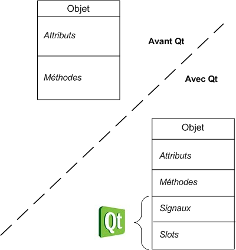
\includegraphics[width=0.6\textwidth]{pictures/sigslot.png}
    \end{frame}
    
    \begin{frame}{Schéma II : pseudo-code}
        \begin{verbatim}{
    public class MaClasse\{ \\ \\
        ~~/* Déclaration attributs */ \\      
        ~~/* Déclaration méthodes */ \\ \\
        ~~public signals:\\
        ~~~~~~void monSignal();\\
        ~~~~~~void monSignal(Type monParam);\\ \\
        ~~public slots:\\
        ~~~~~void monTraitement();\\
        ~~~~~void monTraitement(Type monParam);\\
    \};\\}
    \end{verbatim}
    \\
    \end{frame}
    
    \begin{frame}{Schéma II : pseudo-code (suite)}
    Puis on connecte les signaux aux slots (généralement dans le constructeur) :

   \begin{verbatim}{

    MaClasse()\{ \\ 
    ~~~~...\\
    ~~~~QObject::connect(emeteur, SIGNAL(monSignal()),\\receveur \textit{/* ici this */}, SLOT(monTraitement()));\\ \\
    ~~~~QObject::connect(emeteur, SIGNAL(monSignal(Type)),\\receveur \textit{/* ici this */}, SLOT(monTraitement(Type)));\\
    \} }
    \end{verbatim}
    \\
    \end{frame}
    \begin{frame}{Principe général vs système signaux-slots}
    \begin{itemize}
    \item{La boucle événementielle est appelée par \textit{QApplication::exec()}}
    \item{Les Signaux et les Slots masquent l'existence des \textit{QEvent} (c'est un mécanisme de plus haut niveau).}
    \item{La récupération des messages, leur transformation en signal ou en \textit{QEvent} est transparent pour l'utilisateur.}
    \item{Les Signaux et les Slots permettent de définir facilement le comportement de nos Widgets en fonction des actions de l'utilisateur.}
    \end{itemize}
    \end{frame}
    
    %% Exemple avec vrai code ?
    
    %% Peut être mettre a la place  quelque chose pour annoncer la démonstration? (PS: j'aime vraiment bien la bannière^^)
    
\begin{frame}{Démonstration}
Démonstration !
\end{frame}
    
\begin{frame}{C'est à vous !}
Des questions ?\\
Lancez-vous !
  \end{frame}

\end{document}
